\documentclass[oneside]{report}
\usepackage[utf8]{inputenc}
\usepackage[serbian]{babel}
\usepackage{colortbl}
\usepackage{graphicx}

\graphicspath{ {img/} }

\title{UpamtiOnline - Dokumentacija v.0.$\alpha$}
\author{Lazar Ljubenović \\ Marija Đorđević \\ Miloš Jajac}
\date{Januar 2016}

\usepackage{parskip} % da novi apragraf nema "dva prsta uvučeno" nego da ima razmak između paragrafa
\usepackage{microtype} % bolji paragrafi i hifernacija
\usepackage{tikz}
\usepackage{tikz-uml}

\hyphenation{UpamtiOnline}  % nećemo da se reč UpamtiOnline deli na slogove (ionako će nepravilno da se podeli)ž

\newcommand{\UpamtiOnline}{\textsf{UpamtiOnline}}
\newcommand{\dugme}[1]{\textit{#1}}
\newcommand{\EditCourseButton}{\textit{izmeni kurs}}
\newcommand{\SearchButton}{\textit{pretraži}}
\newcommand{\ChangeAvatarButton}{\textit{promeni avatar}}
\newcommand{\CheckButton}{\textit{check}}
\newcommand{\CrossButton}{\textit{cross}}
\newcommand{\SaveButton}{\textit{snimi}}
\newcommand{\DeleteButton}{\textit{briši}}
\newcommand{\UndoButton}{\textit{briši}}
\newcommand{\PlusButton}{\textit{dodaj}}
\newcommand{\SettingsButton}{\textit{settings}}

\newcommand{\Filename}[1]{\texttt{#1}}

\begin{document}

\maketitle

\part{Vizija sistema}

\chapter{Cilj dokumenta}
Cilj ovog dokumenta je da definiše zahteve koje treba da ispuni aplikacija \UpamtiOnline{}.



\chapter{Opseg dokumenta}
Dokument se odnosi na realizaciju veb aplikacije \UpamtiOnline{}.




\chapter{Reference}
%???




\chapter{Pozicioniranje proizvoda}

\section{Poslovne mogućnosti}
Primarni cilj aplikacije \UpamtiOnline{} je da omogući što adekvatniji proces učenja pojmova uz minimalno uloženo vreme, kao i da korisnicima stvori zabavnu i takmičarsku atmosferu.
Aplikacija treba da obezbedi efikasan sistem za učenje i obnavljanje gradiva, praćenje aktivnosti i napretka korisnika.
Takođe, treba obezbediti jednostavan i intuitivan način za proširenje opsega gradiva aplikacije kako bi korisnici, primenom istog sistema aplikacije, učili gradivo iz željenih oblasti.

\section{Postavka problema}

\begin{center}
    \begin{tabular}{|>{\columncolor[gray]{0.8}}m{2cm}|m{6cm}|}
        \hline
        Problem je &
        Nepostojanje dovoljno efikasnog sistema za učenje pojmova koji se teško pamte a lako zaboravljaju.
        Ovakvi pojmovi su, prvenstveno, reči stranih jezika, imena geografskih pojmova, datumi istorijskih događaja i slični.\\
        \hline
        Pogađa &
        Učenike osnovnih i srednjih škola, studente, ali i ostale ljude koji su zainteresovani da što brže i efikasnije nauče neki strani jezik ili gradivo iz bilo koje druge oblasti interesovanja.\\
        \hline
        Posledice su &
        Naporan i neefikasan proces savladavanja gradiva iz neke oblasti.
        Puno uloženog vremena ali nedovoljno rezultata.
        Konačno, gubljenje interesa i odustajanje od učenja.\\
        \hline
        Uspešno rešenje će &
        Učiniti proces učenja i pamćenja mnogo efikasnijim i zabavnijim uz znatno manje uloženog vremena i napora.\\
        \hline
    \end{tabular}
\end{center}

\section{Postavka pozicije proizvoda}

\begin{center}
    \begin{tabular}{|>{\columncolor[gray]{0.8}}m{2cm}|m{6cm}|}
        \hline
        Za koga &
        Sve ljude koji moraju ili žele da za što manje vremena nauče i u potpunosti savladaju gradivo iz neke oblasti, a pritom žele da proces bude što zabavniji.\\
        \hline
        Proizvod je &
        Veb-aplikacija.\\
        \hline
        Koja &
        Obezbeđuje efikasan sistem za učenje i obnavljanje pojmova kroz sesije koje će trajati ne više od nekoliko minuta, kao i praćenje aktivnosti i napretka korisnika.\\
        \hline
        Za razliku od &
        Postojećih rešenja kojih nema mnogo, nisu dovoljno efikasna ili zabavna.\\
        \hline
        Naš proizvod &
        Omogućuje lako deljenje kurseva za razliku od desktop aplikacija kao npr. Anki, pruža zabavnije i jednostavnije učenje novih pojmova.
        \\
        \hline
    \end{tabular}
\end{center}

\chapter{Opis korisnika}

\section{Opis potencijalnog tržišta}

\section{Profil korisnika}
Postoji samo jedan tip korisnika.
Svi korisnici se registruju i prijavljuju na isti način i imaju iste mogućnosti i privilegije u okviru aplikacije.

\section{Opis okruženja}
Kako je reč o veb-aplikaciji, bilo kom korisniku za rad neophodan je samo računar sa instaliranim veb-pregledačem i internet-konekcijom.
Na ovaj način, korisnik može da se prijavi na svoj nalog sa bilo kog računara koji poseduje pomenuto.

\section{Osnovne potrebe korisnika}
Korisnici treba da imaju mogućnost da uče i obnavljaju gradivo iz različitih oblasti interesovanja.
Takođe, korisnicima treba omogućiti jednostavno dodavanje novog gradiva koje će moći da uče korišćenjem istog sistema.

\section{Alternative i konkurencija}




\chapter{Opis proizvoda}

\section{Perspektiva proizvoda}
Ideja funkcionisanja aplikacije se bazira na sistemu intervalnih ponavljanja (\textit{spaced repetition system}).
To je tehnika učenja koja uključuje rastuće vremenske intervale između uzastopnih obnavljanja prethodno naučenog materijala kako bi se ostvario željeni psihološki efekat.

Mada je princip koristan u raznim kontekstima, obično se primenjuje kada korisnik treba da savlada veliki broj pojmova i da ih na neodređeno vreme zadrži u pamćenju.
Prema tome, tehnika nalazi najveću primenu u obogaćivanju vokabulara korisnika tokom učenja stranog jezika, jer je skup reči neograničeno veliki.

\section{Mogućnosti}

\begin{center}
    \begin{tabular}{|m{3cm}|m{7cm}|}
        \hline
        Koristi korisnika &
        Funkcije proizvoda koje to omogućavaju\\
        \hline
        Učenje pojmova &
        Stranica aplikacije koja sprovodi korisnika kroz sesiju učenja. Sesija obuhvata prikazivanje novih pojmova korisniku i čekanje na njegov odgovor, pritom nudeći mu različite tipove pomoći kako bi korisnik, korak po korak, što lakše savladao gradivo.\\
        \hline
        Obnavljanje pojmova &
        Analogno učenju, korisnik se sprovodi kroz sesiju obnavljanja dela gradiva za koje je već završio fazu učenja. U toku sesije, korisniku se prikazuju pojmovi i aplikacija određeno vreme čeka na odgovor od korisnika. U zavisnosti od tačnosti svakog pojedinačnog odgovora, pojmovi se odlažu određeno vreme, nakon koga će se smatrati da korisnik ponovo treba da ih obnovi.\\
        \hline
        Unos i ažuriranje gradiva &
        Panel aplikacije za kreiranje novih kurseva i unos pojmova omogućava korisniku da na sopstven način organizuje raspored lekcija po svojim kriterijumima i potrebama.\\
        \hline
        Pregled napretka i aktivnosti &
        Indeks stranica korisnika detaljno prikazuje skorašnje informacije o učenju i obnavljanju, kao i informacije o napretku korisnika koje prati.
        \\
        \hline
    \end{tabular}
\end{center}

\section{Pretpostavke i zavisnosti}
Obzirom na to da se radi o veb-aplikaciji, ona može biti pokrenuta sa skoro svakog operativnog sistema, koristeći neku od modernijih verzija veb-pregledača.
Veb-aplikacije je prilagođena većini veličina ekrana, tako da se aplikacije može neometano koristiti kako na desktop računarima, tako i na pametnim telefonima, tabletima, i drugim manjim uređajima.
Stoga, sistem nema većih zavisnosti.

\section{Cena}
Registrovanje naloga, kao i korišćenje svih usluga koje aplikacija pruža je u potpunosti besplatno.

\section{Licenciranje i instalacija}
Aplikaciju nije potrebno instalirati, za korišćenje je dovoljan samo računar sa instaliranim modernim veb-pregledačem i internet-konekcijom.

\chapter{Funkcionalni zahtevi}

\section{Registrovanje korisnika}
Da bi koristio usluge sistema, svaki korisnik mora da bude registrovan, odnosno da ima kreiran nalog. Ovo je neophodno kako bi se identifikovao među ostalim korisnicima i kako bi bilo moguće pamtiti sve potrebne informacije vezane za tog korisnika.

\section{Prijavljivanje korisnika}
Kako bi informacije vezane za nekog registrovanog korisnika mogle da se ažuriraju, potrebno je da on bude prijavljen u trenutku korišćenja sistema.

\section{Učenje gradiva}
\label{sec:ucenje-gradiva}
Učenja novih pojmova treba organizovati u kratke sesije koje će, na više različitih načina, upoznati korisnika sa gradivom i omogućiti mu da ga lako zapamti.

\section{Obnavljanje gradiva}
\label{sec:obnavljanje-gradiva}
Obnavljanje gradiva takođe treba organizovati u sesije koje će biti dostupne korisniku neko vreme nakog učenja tog gradiva. U ovim sesijama se treba ustanoviti koje je pojmove korisnik znao odnosno zaboravio i u zavisnosti od toga treba organizovati buduće sesije obnavljanja.

\section{Kreiranje i ažuriranje kursa}
Ako korisnik ne može naći kurs koji bi hteo da pohađa ili nije zadovoljan gradivom koje je pokriveno, treba mu omogućiti da napravi svoj kurs. Neophodno je obezbediti lak i intuitivan način unosa i organizovanja lekcija i pojmova u okviru novog kursa. Takođe, treba omogućiti ispravljanje i dodavanje novog gradiva.

\section{Dodavanje prijatelja}
Svakom korisniku treba obezbediti mogućnost praćenja aktivnosti drugih korisnika sistema.

\chapter{Ograničenja}
Obzirom na to da se radi o veb-aplikaciji, ona može biti pokrenuta sa skoro svakog operativnog sistema, koristeći neku od modernijih verzija veb-pregledača.
Veb-aplikacije je prilagođena većini veličina ekrana, tako da se aplikacije može neometano koristiti kako na desktop računarima, tako i na pametnim telefonima, tabletima, i drugim manjim uređajima.
Stoga, sistem nema većih ograničenja.

\chapter{Zahtevi u pogledu kvaliteta}
Aplikacija je u stanju da radi dvadeset i četiri časa tokom dana, sedam dana u nedelji, obzirom na to će se izvršavati na moćnom veb-serveru.

\chapter{Prioritet funkcionalnosti}
Funkcionalnost najvišeg prioriteta je prikaz i ispravno funkcionisanje sesija (\ref{sec:ucenje-gradiva} i \ref{sec:obnavljanje-gradiva}), zajedno sa čuvanjem dobijenih podataka u bazi.

\chapter{Nefunkcionalni zahtevi}

\section{Standardi}
Server treba da podrži rad sa SQL bazom, a klijentov veb-pregledač treba da podrži HTML5, CSS3, JavaScript ECMAScript 6.

\section{Sistemski zahtevi}
Ne zahtevaju se računari visokih performansi. Aplikaciju korisnik može da koristi sa bilo kog računara koji ima instaliran moderan veb-pregledač i uspostavljenu internet-konekciju.

\section{Performanse}
Nema posebnih zahteva koji se tiču performansi aplikacije.

\section{Okruženje}
Nema posebnih zahteva u pogledu okruženja.

\part{Specifikacija slučajeva korišćenja}
\label{part:use-case}

\chapter{Uvod}
\label{ch:use-case-uvod}
Slučajevi korišćenja mogu biti podeljeni u sledeće grupe.
\begin{enumerate}
  \item Pristup aplikaciji:
  \begin{enumerate}
    \item Registracija.
    \item Prijava.
  \end{enumerate}
  \item Kursevi:
  \begin{enumerate}
    \item Pretraga kurseva.
	\item Pregled gradiva kursa.
    \item Upis na kurs.
    \item Kreiranje novog kursa.
    \item Ažuriranje kursa.
    \begin{enumerate}
      \item Dodavanje lekcije.
      \item Ažuriranje lekcije.
    \end{enumerate}
    \item Navigacija kroz kurs.
    \item Pregled detaljne statistike.
  \end{enumerate}
  \item Sesije:
  \begin{enumerate}
    \item Učenje.
    \item Obnavljanje.
    \item Spajalica.
  \end{enumerate}
  \item Korisnici:
  \begin{enumerate}
    \item Pregled korisničkog profila.
    \item Praćenje korisnika.
    \item Pregled detaljnih statistika.
  \end{enumerate}
\end{enumerate}



\chapter{Akteri}
\label{ch:akteri}

\section{Korisnik}
\label{sec:korisnik}
Korisnik aplikacije može biti svako lice koje poseduje ispravan računar sa modernim veb-pretraživačem i internet-konekcijom.



\chapter{Slučajevi korišćenja}
\label{ch:slucajevi-koriscenja}

\section{Pristup aplikaciji}
\label{sec:pristup-aplikaciji}
Većina mogućnosti koje aplikacija pruža postaju dostupne korisniku tek nakon registracije, odnosno prijave.

Korisnik koji želi da u potpunosti koristi aplikaciju mora da se registruje na istu (\ref{subsec:registracija}), i po potrebi da se prijavi (\ref{subsec:prijava}).
Ukoliko korisnik trenutno nije prijavljen na aplikaciju, pri njenom pokretanju će dobiti mogućnost registracije i prijave.
Ukoliko je već prijavljen, pri pokretanju aplikacije korisnik vidi svoj profil (\ref{TODO}).

\subsection{Registracija}
\label{subsec:registracija}

\subsubsection{Kratak opis}
Pre početka korišćenja aplikacije korisnik se registruje unošenjem potrebnih informacija. Ovime, korisnik kreira svoj nalog koji će koristiti u daljem radu.

\subsubsection{Osnovni tok događaja}
\begin{itemize}
  \item Posećivanjem početne strane aplikacije pojavljuje se panel za registrovanje.
  \item Korisnik popunjava sva polja neophodna za registrovanje.
  \item Klikom na dugme \dugme{registracija} vrši se upis novog korisnika u bazu.
\end{itemize}

\subsubsection{Alternativni tokovi}
Ako se, nakon klika na dugme \dugme{registracija}, proverom validnosti unetih informacija ustanovi da je došlo do greške, korisnik će biti obavešten kako bi mogao da koriguje unete informacije.
Tek će se nakon ispunjenja svih uslova korisniku odobriti registracija.

\subsubsection{Preduslovi}
Da bi se registracija uspešno obavila, neophodno je ispuniti sva ponuđena polja:
\begin{itemize}
  \item korisničko ime, \item šifra, \item ime i \item mejl adresa.
\end{itemize}

\emph{Korisničko ime} i \emph{mejl adresa} moraju biti jedinstveni u aplikaciji nezavisno jedni od drugog.
Drugim rečima, ne mogu postojati dva naloga sa istim adresama (čak i sa različitim korisničkim imenima), niti dva naloga sa istim korisničkim imenima (čak i sa različitim adresama).
Polja \emph{ime} i \emph{šifra} ne moraju biti jedinstveni za aplikaciju.

\subsubsection{Posledice}
U slučaju uspešnog registrovanja, sistem automatski prijavljuje korisnika na novokreirani nalog i otvara njegovu indeks stranicu, u suprotnom se od korisnika traži da ponovi pokušaj registrovanja.


\subsection{Prijava}
\label{subsec:prijava}

\subsubsection{Kratak opis}
Ako korisnik ima nalog a nije prijavljen, korisnik se prijavljuje na svoj nalog pre korišćenja aplikacije.

\subsubsection{Osnovni tok događaja}
\begin{itemize}
  \item Posećivanjem početne strane aplikacije pojavljuje se panel za prijavljivanje.
  \item Korisnik popunjava sva polja neophodna za prijavljivanje.
  \item Ako želi, štiklira polje \emph{zapamti me}.
  \item Klikom na dugme \dugme{prijava} sistem pretražuje unete informacije u bazi i prijavljuje korisnika.
\end{itemize}

\subsubsection{Alternativni tokovi}
Ako se, nakon klika na dugme \dugme{prijavi}, proverom validnosti unetih informacija ustanovi da je došlo do greške, korisnik će biti obavešten kako bi mogao da koriguje unete informacije.
Tek će se nakon ispunjenja svih uslova korisniku odobriti prijavljivanje.

\subsubsection{Preduslovi}
Da bi se prijavljivanje uspešno obavilo, neophodno je ispuniti ponuđena polja \emph{korisničko ime} i \emph{šifra}.

\emph{Korisničko ime} mora postojati u bazi aplikacije i \emph{šifra} mora biti odgovarajuća kako bi se dozvolilo prijavljivanje korisnika.

\subsubsection{Posledice}
U slučaju uspešnog prijavljivanja korisniku će se otvoriti indeks stranica njegovog naloga, u suprotnom će se od korisnika tražiti da ponovi pokušaj prijavljivanja.





\section{Kursevi}
\label{sec:kursevi}
Kursevi su glavna jedinica organizacije gradiva.
Svim posetiocima treba obezbediti pretragu svih postojećih kurseva koji su organizovani u kategorije i detaljan pregled njihovog sadržaja.
Ako posetilac ima nalog i ako je prijavljen, ima mogućnost da se upiše na neki kurs i tako postane učesnik.
Svi prijavljeni korisnici takođe mogu da kreiraju svoje kurseve i da ih ažuriraju.

\subsection{Pretraga kurseva}
\label{subsec:pretraga-kurseva}

\subsubsection{Kratak opis}
Pretraživanje kurseva aplikacije po unetim kriterijumima.

\subsubsection{Osnovni tok događaja}
Korisnik, na stranici pregleda kurseva, unosi ime ili deo imena kursa koji hoće da nađe u polje \emph{naziv} i opciono bira kategoriju i potkategoriju u kojoj će se vršiti pretraga željenog kursa.
Nakon toga, klikom na dugme \SearchButton vrši se pretraga i prikazuje se lista kurseva koji odgovaraju unetim kriterijumima.

\subsubsection{Alternativni tokovi}

\subsubsection{Preduslovi}

\subsubsection{Posledice}
Kako na stranici pregleda kurseva korisnik može da vidi sve kurseve koji postoje u aplikaciji, nako pretrage lista prikaza se redukuje samo na kurseve koji zadovoljavaju kriterijume pretrage.


\subsection{Pregled gradiva kursa}
\label{subsec:pregled-gradiva-kursa}

\subsubsection{Kratak opis}
Evaluacija gradiva koje neki kurs pokriva.

\subsubsection{Osnovni tok događaja}
Korisnik, klikom na dugme \dugme{spisak} za odgovarajuću lekciju u kursu, otvara prozor koji prikazuje informacije vezane za tu lekciju.

\subsubsection{Alternativni tokovi}

\subsubsection{Preduslovi}

\subsubsection{Posledice}



\subsection{Upis na kurs}
\label{subsec:upis-na-kurs}

\subsubsection{Kratak opis}
Korisnik se upisuje na kurs kako bi mogao da uči i obnavlja gradivo koje taj kurs sadrži.

\subsubsection{Osnovni tok događaja}
Na stranici kursa klikom na dugme \dugme{upiši se}, korisnik se upisuje na dati kurs, odnosno postaje učesnik tog kursa.

\subsubsection{Alternativni tokovi}

\subsubsection{Preduslovi}
Korisnik mora biti prijavljen kako bi mu se na stranici kursa prikazalo dugme \dugme{upiši se}.

\subsubsection{Posledice}
Nakon upisa na kurs, korisniku su omogućene opcije za učenje i obnavljanje lekcija tog kursa.



\subsection{Kreiranje kursa}
\label{subsec:kreiranje-kursa}

\subsubsection{Kratak opis}
Korisnik kreira novi kurs koji će samo on moći da ažurira.

\subsubsection{Osnovni tok događaja}
\begin{itemize}
  \item Korisnik unosi naziv kursa koji će da kreira i kategoriju kojoj će taj kurs da pripada.
  \item Ako želi i ako odgovarajuća potkategorija postoji, može izabrati i potkategoriju.
  \item Klikom na dugme \dugme{kreiraj} vrši se upis potrebnih informacija u bazu.
\end{itemize}

\subsubsection{Alternativni tokovi}
Ako korisnik nije uneo naziv kursa ili nije odabrao kategoriju, dobiće odgovarajuću poruku.

\subsubsection{Preduslovi}

\subsubsection{Posledice}
Nakon uspešnog kreiranja novog kursa, automatski se otvara stranica za ažuriranje tog kursa.


\subsection{Ažuriranje kursa}
\label{subsec:azuriranje-kursa}

\subsubsection{Kratak opis}
Kreator kursa vrši ažuriranje informacija koje su vezane za kurs i za lekcije koje pripadaju tom kursu.
Nakon unošenja svih potrebnih izmena potrebno je kliknuti na dugme \SaveButton{} čime se završava ažuriranje.

\subsubsection{Osnovni tok događaja}
\begin{itemize}
  \item Na stranici kursa, kreator klikom na dugme \EditCourseButton{} otvara stranicu za ažuriranje kursa.
  \item Klikom na ime kursa omogućeno je kucanje novog imena. Nakon izmene, klikom na \CheckButton se potvrdjuje promena imena. Klikom na \CrossButton novo ime se odbacuje i kurs zadržava prvobitno ime.
  \item Klikom na dugme \EditCourseButton{} za opis kursa moguće je ažurirati njegov opis. Nakon izmene, klikom na \CheckButton se potvrdjuje promena opisa. Klikom na \CrossButton novi opis se odbacuje i kurs zadržava prvobitni opis.
  \item Klikom na dugme \ChangeAvatarButton{} otvara se standardni meni za izbor nove slike. %ovde možda da se doda ono klikom na choose file pa na upload pa bla bla
  \item Nakon željenih izmena, klikom na dugme \SaveButton{} se potvrdjuju unete izmene i nove informacije o tom kursu su sada sačuvane.
\end{itemize}
\subsubsection{Alternativni tokovi}
Ako nakon izmena nove informacije nisu validne, klikom na dugme \SaveButton{} neće biti ažurirane informacije o kursu i korisniku će se prikazati poruka kako čuvanje novih informacija nije bilo uspešno.
\subsubsection{Preduslovi}
Da bi korisnik uopšte mogao da pristupi stranici za ažuriranje kursa, on mora biti kreator tog kursa.
\subsubsection{Posledice}
Nove informacije o kursu koje je korisnik uneo se čuvaju u bazi i ovime je završen proces ažuriranja.

\subsection{Kreiranje lekcije}
\label{subsec:kreiranje-lekcije}

\subsubsection{Kratak opis}
Korisnik dodaje novu lekciju u neki od svojih kurseva.

\subsubsection{Osnovni tok događaja}
\begin{itemize}
  \item Na stranici kursa, kreator klikom na dugme \PlusButton{} započinje pravljenje nove lekcije.
  \item Korisnik zatim unosi ime nove lekcije.
  \item Ponovnim klikom na dugme \PlusButton{} potvrđuje kreiranje lekcije sa unetim imenom.
\end{itemize}
\subsubsection{Alternativni tokovi}
Ako korisnik nije uneo naziv lekcije ili lekcija sa unetim nazivom već postoji u okviru tog kursa, dobiće odgovarajuću poruku.
\subsubsection{Preduslovi}
Da bi kreiranje lekcije bilo uspešno, u okviru tog kursa ne sme već postojati lekcija sa istim imenom.
\subsubsection{Posledice}
Nakon uspešnog kreiranja, nova lekcija se automatski dodaje na listu postojećih lekcija tog kursa i može se vršiti njeno ažuriranje.


\subsection{Ažuriranje lekcije}
\label{subsec:azuriranje-lekcije}

\subsubsection{Kratak opis}
Korisnik vrši izmenu informacija o samoj lekciji ili o pojmovima koji se uče unutar te lekcije.
Nakon unošenja svih potrebnih izmena potrebno je kliknuti na dugme \SaveButton{} čime se završava ažuriranje.

\subsubsection{Osnovni tok događaja}
\begin{itemize}
  \item Klikom na dugme \SettingsButton{} otvara se padajući meni koji nudi više opcija za ažuriranje:
  \begin{itemize}
    \item \emph{Promeni ime} dozvoljava korisniku da unese novo ime lekcije.
    Novo ime se potvrdjuje klikom na \CheckButton{} ili poništava klikom na \CrossButton{}.
    \item \emph{Obriši lekciju} u potpunosti briše sve informacije vezane za tu lekciju kao i za sve pojmove unutar lekcije.
    \item \emph{Grupno menjanje} dozvoljava korisniku da ažurira informacije o bilo kom pojmu u toj lekciji.
    Sve izmene se istovremeno potvrđuju klikom na \CheckButton{} ili poništavaju klikom na \CrossButton{}.
    \item \emph{Zameni pitanje i odgovor} će, za svaki pojam unutar te lekcije, međusobno zameniti informacije zapisane u poljima \emph{pitanje} i \emph{odgovor}.
    \item \emph{Promeni opis svima} omogućava korisniku da istovremeno promeni opis svim pojmovima unutar te lekcije. % ovde da se doda nešto ako treba kad ga laza promeni
  \end{itemize}
  \item Klikom na sličicu pored imena nivoa otvara se padajući meni različitih sličica i boja koje korisnik može odabrati.
  \item Dodavanje novog pojma započinje klikom na \PlusButton{} u okviru lekcije.
  Zatim se vrši unos informacija u polja \emph{pitanje}, \emph{odgovor} i \emph{opis}, a zatim ponovnim klikom na \PlusButton{} se potvrđuje dodavanje novog pojma.
  \item Ažuriranje postojećeg pojma se vrši klikom na \EditCourseButton za odgovarajući pojam.
  Nakon izmene željenih informacija korisnik potvrđuje izmene klikom na \CheckButton{} ili ih poništava klikom na \CrossButton{}.
  \item Brisanje postojećeg pojma se vrši klikom na \DeleteButton{} za odgovarajući pojam.
  Nakon ovoga, ako korisnik želi da poništi brisanje, to može uraditi klikom na \UndoButton{}.
  \item Kada korisnik završi sa ažuriranjem lekcije, klikom na \SaveButton{} potvrđuje sve izmene i baza se ažurira.
\end{itemize}
\subsubsection{Alternativni tokovi}
Ako informacije vezane za lekciju nakon izmena nisu validne, klikom na dugme \SaveButton{} ažuriranje baze se neće izvršiti i korisnik će biti obavešten odgovarajućom porukom.
\subsubsection{Preduslovi}

\subsubsection{Posledice}
Nove informacije o lekciji koje je korisnik uneo se čuvaju u bazi i ovime je završen proces ažuriranja.

\subsection{Navigacija kroz kurs}
\label{subsec:navigacija-kroz-kurs}

\subsubsection{Kratak opis}
Akcije koje korisnik može započeti u okviru kursa.
\subsubsection{Osnovni tok događaja}
\begin{itemize}
  \item Klikom na dugme \dugme{uči} korisnik započinje sesiju učenja podrazumevanog broja novih pojmova.
  Opciono, korisnik može klikom na padajući meni na istom dugmetu da promeni broj pojmova koje želi da uči u jednoj sesiji.
  \item Klikom na dugme \dugme{obnovi} korisnik započinje sesiju obnavljanja podrazumevanog broja pojmova.
  Opciono, korisnik može klikom na padajući meni na istom dugmetu da promeni broj pojmova koje želi da obnavlja u jednoj sesiji.
  \item Klikom na dugme \dugme{spajalica} korisnik započinje sesiju igre \emph{spajalica}.
\end{itemize}
\subsubsection{Alternativni tokovi}

\subsubsection{Preduslovi}
Korisnik mora biti prijavljen i mora biti učesnik na tom kursu kako bi imao ponuđene pomenute opcije.
\subsubsection{Posledice}



\subsection{Učenje}
\label{subsec:ucenje}

\subsubsection{Kratak opis}

\subsubsection{Osnovni tok događaja}

\subsubsection{Alternativni tokovi}

\subsubsection{Preduslovi}

\subsubsection{Posledice}




\subsection{Obnavljanje}
\label{subsec:obnavljanje}

\subsubsection{Kratak opis}

\subsubsection{Osnovni tok događaja}

\subsubsection{Alternativni tokovi}

\subsubsection{Preduslovi}

\subsubsection{Posledice}




\subsection{Spajalica}
\label{subsec:spajalica}

\subsubsection{Kratak opis}

\subsubsection{Osnovni tok događaja}

\subsubsection{Alternativni tokovi}

\subsubsection{Preduslovi}

\subsubsection{Posledice}



% ovde vrv nece bude nista na kraju? msm sta, samo gledas profil, nema neke interakcije
\subsection{Pregled korisničkog profila}
\label{subsec:pregled-korisnickog-profila}

\subsubsection{Kratak opis}

\subsubsection{Osnovni tok događaja}

\subsubsection{Alternativni tokovi}

\subsubsection{Preduslovi}

\subsubsection{Posledice}




\subsection{Praćenje korisnika}
\label{subsec:pracenje-korisnika}

\subsubsection{Kratak opis}
Korisnik počinje da prati aktivnost drugog korisnika.
\subsubsection{Osnovni tok događaja}
Prijavljen korisnik koji se trenutno nalazi na stranici profila nekog drugog korisnika, klikom na dugme \dugme{prati} počinje da prati aktivnost tog korisnika.
\subsubsection{Alternativni tokovi}

\subsubsection{Preduslovi}

\subsubsection{Posledice}
%ovde nesto tipa sad kad ga prati ga vidi na rang listi na svojoj indeks strani al jebem li ga da l' to treba ovde uopste da se pise

\part{Arhitektura softvera i detaljno projektovanje}

\chapter{Kratak opis}
Dokument obrađuje pregled arhitekture aplikacije \UpamtiOnline.

\chapter{Reference}
Pogledati:
\begin{enumerate}
  \item Specifikacija slučajeva korišćenja (\ref{part:use-case}) aplikacije \UpamtiOnline.
\end{enumerate}

\chapter{Reprezentacija arhitekture}
Arhitektura sistema u dokumentu je prikazana kao serija pogleda na sistem:
pogled na slučajeve upotrebe, pogled na procese, pogled na primenjeni sistem i pogled na implementaciju.
Ovi pogledi su grafički predstavljeni kao modeli pomoću jezika UML.

\chapter{Ciljevi arhitekture}

Arhitektura je dizajnirana uzimajući u obzir sledeće:
\begin{enumerate}
  \item Korisnički interfejs je pažljivo dizajniran da bi bio jednostavan i intuitivan za korišćenje.
  \item Sve akcije koje mogu dovesti u pitanje konzistentnost i validnost podataka moraju biti programski onemogućene; na primer: na istom kursu se ne mogu naći dve kartice sa identičnim pitanjem; ne sme postojati prazna lekcija ili kurs, itd.
  \item Program mora da održava vremensku konzistentnost podataka koji se unose i obrađuju, i to pomoću mehanizama koji nisu vezani za korisnika programa.
  \item Program mora da na efikasan način radi sa velikim brojem kurseva odnosno kartica koje koristnici uče.
\end{enumerate}

\chapter{Pogled na slučajeve upoterbe}
Slučajevi korišćenja mogu biti podeljeni u grupe kao što je to učinjeno u \ref{ch:use-case-uvod}.

\section{Slučajevi upotrebe značajni za arhitekturu sistema}
% kad ih ajjac napise referenciraj

\chapter{Pogled na logičku predstavu sistema}

\section{Pregled arhitekture -- paketi, podsistemi i slojevi}

Sistem se sastoji od tri podsistema (vidi sliku \ref{fig:paketi}):
\begin{itemize}
  \item sloj podataka,
  \item logika sistema,
  \item interfejs.
\end{itemize}

\begin{figure}[htbp]
  \centering
  \begin{tikzpicture}
    \begin{umlpackage}[x=0, y=8]{korisnicki interfejs}
    \end{umlpackage}
    \begin{umlpackage}[x=0, y=4]{logika aplikacije}
    \end{umlpackage}
    \begin{umlpackage}[x=0, y=0]{sloj za prisup podacima}
    \end{umlpackage}
    \begin{umlpackage}[x=5, y=0]{baza}
    \end{umlpackage}
    \umlimport{korisnicki interfejs}{logika aplikacije}
    \umlimport{logika aplikacije}{sloj za prisup podacima}
    \umlimport{sloj za prisup podacima}{baza}
  \end{tikzpicture}
  \caption{Pregled arhitekture: paketi, podsistemi i slojevi}
  \label{fig:paketi}
\end{figure}

Sloj podataka predstavlja projekat \Filename{Data} koji služi za komunikaciju sa bazom podataka i sadrži odgovarajući API.

Logika sistema je realizovana u projektu \Filename{UpamtiMe}, koji je MVC veb-aplikacija koja se oslanja na ASP.NET frejmvork.

Interfejs sistema je realizovan kao skup HTML5 dokumenata, pisanih kao \Filename{.cshtml} pomoću Rejzorove sintakse.
Za dizajn je korišćen CSS3, generisan pomoću skript-jezika SASS i sintakse SCSS.
Za interakciju sa korisnikom, kao i asinhrono komuniciranje sa samom aplikacijom korišćen je JavaScript, i njegov frejmvork jQuery.

\chapter{Pogled na implementaciju}

\section{Baza podataka}
Slika \ref{fig:sema-baza} predstavlja bazu podataka na koju se oslanja aplikacija \UpamtiOnline.

\begin{figure}[htbp]
  \centering
  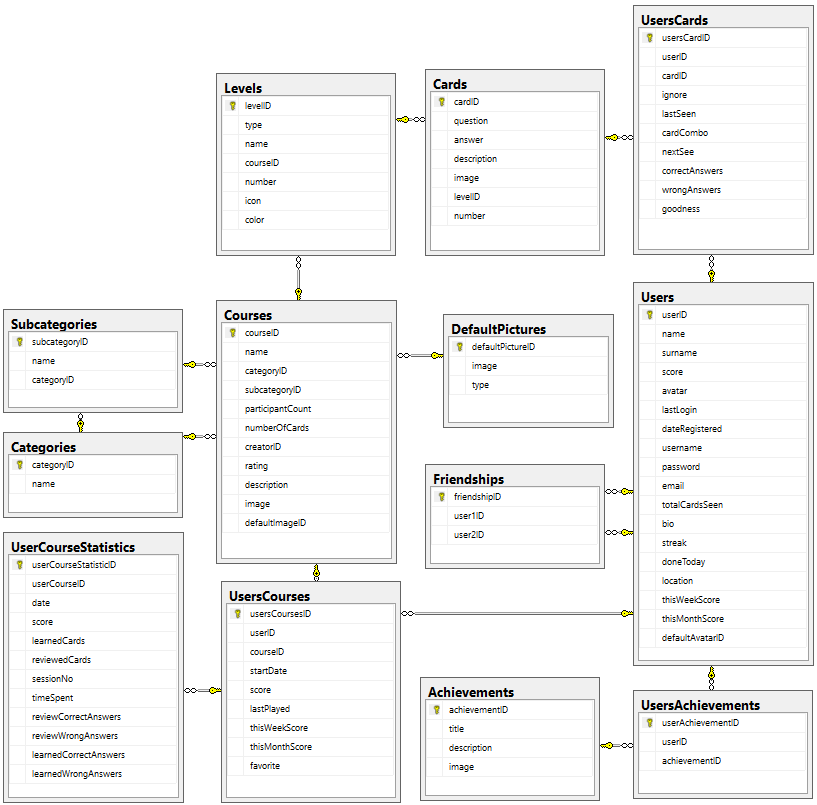
\includegraphics[scale=0.55]{baya}
  \caption{Šema baze podataka}
  \label{fig:sema-baza}
\end{figure}

\section{Sesije}
Sesija se, nezavisno od toga da li je u pitanju sesija učenja ili sesija obnavljanja, sastoji od više različitih izazova (igara).
Da bi sesija mogla da se sastoji od proizvoljnih izazova, i kako bi eventualno buduće dodavanje novih izazova u sistem bilo moguće obaviti na jednostavan način, prilikom implementacije upotrebljeni su projektni obrasci, među kojima su Unikat, Strategija i Posmatrač.

Sama sesija je implementirana kao Unikat i sadrži raspored kartica, pri čemu svaka kartica ima niz pokazivača na strategije, koje su zapravo izazovi.
Svaka strategija ima jedinstven način prikaza i neophodne podatke (na primer, izazov Hangman sadrži string u kome su samo pojedina slova prikazana).
Prilikom pokretanja sesije, na slučajan način se generiše raspored kartica, a redosled strategija svake kartice ostaje nepromenjen.

Kada korisnik tokom sesije da tačan odgovor, ta kartica prelazi na sledeću strategiju, koja će biti prikazana kada ta kartica dođe na red.
Ukoliko korisnik da netačan odgovor, strategija odgovarajuće kartice ostaje nepromenjena kako bi se ona ponovo prikazala kada sledeći put pomenuta kartica dođe na red, ali se kartica istovremeno odlaže i na kraj rasporeda.
Na taj način na pogrešeno pitanje dogovor daje više puta, kako bi se pojam urezao u korisnikovo pamćenje.

\input{8-korisnicko-upustvo}

\end{document}
